
\chapter{Medication reconciliation}

The free-text medication data in Electronic Health Records (EHRs) is predominantly unsanitised, and its unstructured nature makes it inaccessible to other computer applications that rely on coded data in healthcare settings (e.g, electronic medication reconciliation systems), as well as clinical research that uses structured medication data, such as EHR-based\cite{kushima2012text}. Despite providing a means of reducing paper-based inaccuracy, Electronic Medical Record Management systems are still subject to human error \cite{koppel2009emr}.

Medication reconciliation is a formal process for creating a more complete and accurate list of a patient's medications for the purpose of supporting correct medication orders. Given the increasing use of EHRs, automated medication reconciliation methods have received great attention\cite{grossman2014hospital}. One particular challenge involves the heterogeneity of clinical data, which consists of both coded and narrative medical data.\cite{michaelsen2015medication}

Despite the inherent value that these terms bear, free-text medical information may contain large volumes of pharmaceuticals recorded inconsistently, both stylistically and structurally. The pharmaceuticals themselves may be incorrectly recorded, and no list of pharmaceuticals likely to recorded in a corpus may exist. The purpose of this paper is to develop a system that can extract drug names from this unstructured data in order that this information be available for analytical purposes, both on a population and individual basis. In this way it may be possible to provide useful and interesting inferences over large volumes of data.

This research will be using a corpus of 211000 cases treated in 2014 in an Out-of-Hours (OOH) general practitioner cooperative in Ireland \cite{natreview}. Electronic Health Records used in the operation of OOH coops are composed of both normalised and free-text clinical notes. The EHR software used by the co-op and the majority of OOH medical providers within Ireland and Great Britain is Ad Astra\textsuperscript{TM} \cite{natreview}.  

This paper will examine the ways in which pharmaceutical discovery can be achieved, before looking at extant research into the area. The proposed solution will focus on environmental analysis of the text and, as such, a section will explore the manner in which this was conducted. Finally, the results of the information retrieval and success of the clustering of such terms is analysed.   



\section{Problem Definition}

 While drug names tend to follow certain morphological conventions, these not only pose a problem by their sheer volume, but even presupposing that pharmaceuticals are recorded using full international non-proprietary name \\ (INN),\cite{dunne2013review} stems used to denote drugs are syntactically so sparse as to preclude any sort of acceptable precision. Naturally, such affixes and suffixes are unlikely to relate to proprietary names under which these products are marketed, which may be the manner in which drug products are represented within the text. As such, the analysis of words, in isolation, to discover medications within the text can be discounted. 
 

Instead, an analysis of the structure of medical notes to detail the types of syntax which are likely to indicate the presence of medications will be conducted. Although the heterogeneity of free-text notes precludes certain Natural Language Processing (NLP) measures, developing simple syntactic patterns has the potential to accurately return medication names within such notes.

It is a primary ambition of this paper to deliver a system that can not only identify the proprietary, trade and generic names of pharmaceuticals, but provide also the means for incorrectly transcribed pharmaceuticals occurring within free-text notes to be automatically corrected with a high degree of precision. 

This paper aims to discover a broad spectrum of medications, but will consider all other lexicons to be incorrect. For instance, the term ``antibiotic" would be considered to be a valid medication name (despite its generic nature) while a word like ``emulsion", which denotes a delivery method for medications, would be considered incorrect. All lexicons which denote medications, but are incorrectly spelled (for instance prendnesol instead of prednesol) will be considered erroneous.  

\section{Proposed Solution}

Using a predefined list of drug names, co-occurring terms found within the text will be collected, excluding stop words.  The highest frequencies of co-occurring lexemes will next be compared against one another in order to develop well defined environments within which medications are likely to be present. 

Once structures which telegraph the presence of medication details have been defined, suitable structures will be used to collect lexemes which may represent medications.  The data collected will exclude common English words and lexemes less than three characters in length. The accuracy of the pattern used to discover candidate medications names will underpin the precision of the overall program, as both unrelated medical words, and misspelled words that do not relate to medications are otherwise likely to be returned by this process.

By searching all other text for occurrence of the collected words, a dataset of pharmaceuticals and their frequency within the EHR can be established. Data relating to common English words is derived from a truncated version of SCOWL (Spell Checker Oriented Word Lists), totalling some 50000 words. The collection of drug and product names above is guaranteed to return many errors, both typographical and cognitive in nature, where users have entered the names of products they are describing incorrectly. Common English words which have been misspelled, and domain-specific terms alike may also hypothetically be collected in this process. Furthermore, terms that are four characters in length are overwhelmingly likely to represent domain-specific acronyms, or product name contractions. However, by analysing both the frequency of occurrence and morphological similarity of the terms collected, it is intended that the program will automatically correct these errors.
 




%\begin{figure}[!t]
%\centering
%\includegraphics[width=2.5in]{workflow.png}
%% where an .eps filename suffix will be assumed under latex, 
%% and a .pdf suffix will be assumed for pdflatex; or what has been declared
% \DeclareGraphicsExtensions.
%\caption{Overall program structure.}
%\label{workflow}
%\end{figure}


\section{Related Work}
Despite the dirty nature of free-text and colloquial language often used, the domain specific nature means that many of the issues surrounding the investigation of other media for medical related phenomena (such as those experienced by Michael J et al when treating Twitter data for disease related terms)\cite{paul2012model} are circumvented.

Nevertheless, the same general problems repeatedly arise when approaching clinical notes: the presence of both semi-structured and unstructured textual data (the latter of which contains high value domain terms), the relationship these terms have upon each other in free-text environments, and the means by which this data can be transformed in order to provide meaningful analysis. To date, medications have predominantly been discovered in text through use of comprehensive predefined lists, though some work may be done to overcome the shortcomings of such an approach. 

Levin et al. look at the issue of discovering drug names in free text relating to preoperative drug history contained within anaesthesiologist EHRs \cite{levin2007extraction}. Levin et al. used the RxNorm lexicon of clinical drug nomenclature in order to find drug names within the dataset. This list approach is used extensively, with a variant of Soundex applied in order to increase recall of pharmaceuticals. This approach seems partially inspired by the overarching design to match proprietary names to generic equivalents. Ultimately, Levin et al. achieve an exceptionally high PPV (Positive predictive value) of 98.8\% but a decidedly more modest NPV (Negative Predictive Value) of 76.2\%. 

Hua Xu et al. also base their system largely off of RxNorm, and supplemented their findings using a regular expression tagger \cite{xu2010medex}. Filtering of English words in this system is based upon the SCOWL list. The system that Hua Xu et al employ requires some manual review of ambiguous terms to be conducted by a physician, but seems to have some capacity to handle abbreviations that are hitherto unknown by the system. However, the exact means by which abbreviations are mapped to their longer forms is not explored.  Results comparable with Levin et al.'s paper were achieved with an F-measure of 92\% on clinical notes. 

Yan Xu et al. were among many who used the 2010 i2b2 dataset to further investigation into the processing of medicinal textual data\cite{xu2012named}. Unlike some other research, the annotations supplied with the dataset were used solely for testing purposes by Xu et al. As such, one of the primary ambitions of the research lay on the successful extraction of medical concepts within the free text notes of the i2b2 dataset. 

Although the i2b2 2010 challenge established the named-entities of ``medical", ``problem", ``treatment", and ``test", Xu et al. identified that members of these classes did not necessarily appear in a similar manner to one another. In particular, Xu et al established a sub-class of "treatment" relating to medication, due to the fixed distinct semantic pattern that pharmaceuticals tended to take within the corpus. Consequently, an elaborate regular expression solution was built to capture these particular concepts.    

Attempts to define medications purely through use of a predefined ontology (namely UMLS) fared poorly for Xu et al. due to the abundance of lexical variations that medications were subject to. Due to the variety of trade names and synonyms, Xu et al declare that it may be ``impossible'' to construct a dictionary that will reflect this plurality yet reliably stay up-to-date. 


Xu et al. attempted to deal with the ambiguity of acronyms and abbreviations by unsupervised clustering both types of contraction into their respective classes (i.e. ``medical'', ``problem", ``treatment", and ``test"). This clustering was based upon the distributional and morphological information of the lexemes. This is, however, confusing, as the means of discovering such lexemes is not described, and acronyms and abbreviations by their nature tend to offer poor morphological information.  

While clear that rule based systems are a crucial part of the solution provided, Xu et al. elaborate that the output of the rule based systems was not an end product in itself. Rather, the output from these rules was fed to classifiers, the result of which is used to achieve the aims of the i2b2 challenge. Fundamentally however, Xu et al. demonstrated that the switch to a model which extracted treatments by looking for telegraphic sentences greatly improved feature extraction when it came to medicines mentioned within the text. 
\\

\section{Methodology} 
 
%The data provided, which had previously been anonymised, was cleaned of duplicate entries and tokenised. The preprocessed text was analysed for sentence structures which would indicate the presence of prescription details. Terms in proximity to numerical tokens succeeded by prescription related lexemes were collected as candidate names.

By taking the list of drugs presented within RxNorm, the frequencies of all co-occurring words were recorded. Co-occurring words could appear immediately before or after the name being searched, provided that it was not interceded by punctuation (newlines, periods, etc.). Stopwords were excluded from this process using the twenty five semantically non-selective words which are common in Reuters-RCV1.\cite{sanderson2010christopher} 

Having collected the frequencies of co-occurring words, work was begun on creating a co-occurrence network in order to identify structures within the text that pharmaceuticals are likely to be found. Analysis of the interconnection between the top forty terms was conducted. Interconnection was determined by simultaneous presence of terms on the same line of text within the corpus of free-text notes. 

The co-occurrence network eliminated nodes that failed to have any edge with a weight within the top half of occurrences. Finally, modularity of the network was conducted, separating the network into three distinct classes using Blondel et al.'s clustering algorithm,\cite{blondel2008fast} as can be seen below. Some terms that have have particularly strong connections to other clusters are not considered mutually exclusive (e.g. `pain' is considered to be in both the green and orange clusters).

The orange coloured community represents paediatric related contexts. Nurse triages answering paediatric related cases may advise the use of non-prescription based medicines in many cases in order to ease the symptoms relating to the child's complaint. This context consequently tends towards a relatively limited number of medications which occur in high frequency. This can be observed in the presence of a pharmaceutical name which has actually appeared within this cluster (namely `calpol').

The second community identified (green) is a more generalised context relating principally to initial contact between a patient and phone operator where non-specific details may be related. While the lexemes in this group have a relatively strong correlation with medications, and a particularly high correlation with one another, the high variance of types of information related in the proximity of these terms augurs poorly for the precision of medicine based information retrieval. 

Prescription details (purple) closely mirror their real-world handwritten equivalents, both in terms of register and structure. As such, the invocatio of the praescriptio typically contains weights and measures \cite{hadavsova2009practicals}. This generates a consistent pattern of drug or product names, succeeded by measurements (that may change temporally), which may be followed by some temporal value. These prescription details may be singular or composite.

When looking for non-lexical co-relation with the different classes, prescription based words had a particularly strong relationship with numerical elements. Lexicons belonging to the prescription class had a total of 100669 numerical co-occurrences compared with 3654 for general and 12954 for paediatric contexts. 

Taking account of the semantic ordering of prescription related terms, certain patterns became apparent, with particular terms tending towards different relative positions. When grouping the terms by meaning (relating to quantifiable and temporal specifications), the most common semantic structure was for numerical tokens to be followed by quantification and temporal tokens, in that order (with some 25618 occurrences). The second most common structure was for numerical tokens to be followed simply by quantification tokens (with some 16617 occurrences).  

Using this as a means by which to proceed, the preprocessed text of the corpus was analysed for sentence structures which would indicate the presence of prescription details. Terms in proximity to numerical tokens, succeeded by prescription related lexemes in the order hitherto observed, were collected as candidate names. Terms which were within SCOWL were excluded, while those less than three characters in length were discarded in favour of the nearest suitable lexeme. 

%test
\begin{figure}
\centering
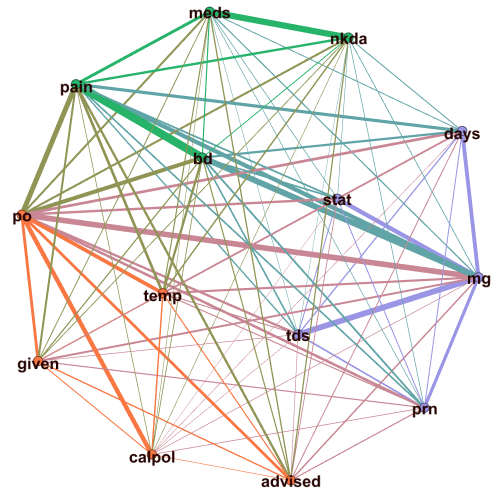
\includegraphics[width=2.5in]{relations.png} %testucd
% where an .eps filename suffix will be assumed under latex, 
% and a .pdf suffix will be assumed for pdflatex; or what has been declared
\DeclareGraphicsExtensions.
\caption{Undirected graph of context relations.}
\label{regex}
\end{figure}


%In order to determine the accuracy of the program an exhaustive search was conducted through various media to ascertain whether each of the recorded candidate names was a correctly written pharmaceutical. 

Following the collection process, a frequency was taken of all collected candidate names within the entire training corpus. This was done so that the recorded frequency would reflect the general preponderance of candidate names within the text, not limited solely to the context of prescriptions.

Of the terms collected, names that were were exactly four characters in length overwhelmingly represented false positives or abbreviated forms of drug names. Contracted forms of drug names typically have very large edit distances from their full length versions, so a specific process of contraction inflation was developed. This process analysed the longer candidate medication names for a potential match, based both upon length and morphological similarity. In the event of a conflict, the full-length candidate name with a greater frequency was chosen. Any term which ultimately found no suitable match was removed from the list of candidate names.

Finally, the edit distance between candidate pharmaceuticals was tested using an implementation of the Levenshtein distance string metric.\cite{schulz2002fast} The hypothesis was developed that supposed that the edit distances would be predominantly short between incorrect pharmaceutical entries and their correct versions, and that, as a general principle, incorrect edits would necessitate longer edit distances.\cite{hodge2003comparison}  This was implemented using varying distance criteria, and the results recorded.


%\begin{figure}
%\begin{algorithmic}[1]
%\Procedure{editDistance}{$s1,s2$}
%\State $a[i,k] =0$
%\For{$i = 1 \to  |s1|$}
%\State {$a[i,0] = i$}
%\EndFor
%\For{$k = 1 \to  |s2|$}
%\State {$a[0,k] = k$}
%\EndFor
%\For{$i = 1 \to  |s1|$}
%    \For{$k = 1 \to  |s2|$}
%    \State {$a[i,k] = \min\{a[i-1,k-1]+$}
%    \If{$(s1[i]=s2[k])$}
%        \State{$0$} 
%    \Else 
%    \State{$1$} 
%    \EndIf
%    \State {$a[i-1,k]+1, a[i,k-1]+1$}
%    \EndFor
%\EndFor
%\label{euclidendwhile}
%\State \textbf{return} $a[|s1|,|s2|]$
%\EndProcedure
%\end{algorithmic}
%\caption{Levenshtein distance}\label{euclid}
%\end{figure}


\section{Results}

Candidate medications were collected from the dataset through the identification of prescription details. This resulted in 3778 candidate pharmaceutical names being obtained. When searched for through the entire corpus, it was found that these candidate names related to some 460232 occurrences within the entire text.  

However, of these candidate names, only 896 terms were correct. Of the 2893 incorrect candidate names, the vast majority represented incorrectly spelled drug names, with only 98 falling into other categories (predominantly relating to abbreviated forms of drugs and routes of administration). Incorrect terms accounted for roughly half the population of candidate instances within the corpus (152500 versus 155295).


\subsection{Abbreviation inflation}

The abbreviation inflation program was run on the 86 candidate names which were 4 characters in length. This resulted in one false-negative being deleted (a drug with some 569 occurrences in the corpus), and two false-positives, where drugs were wrongly inflated to larger forms (accounting for 17 occurrences together). 

Twenty-eight true-positives were identified and correctly inflated (totalling some 2990 occurrences), although two of these candidates were inflated to words which were themselves incorrect candidates.%: namely nebulizer (61) and suppository (52), both of which are routes of administration rather than pharmaceuticals.

An additional fifteen abbreviations (totalling 89 occurrences) were incorrectly identified as being pharmaceutical abbreviations and were added to the count of extant drugs.

Forty-two abbreviations were deleted, thirty eight of which were correctly identified as being unrelated to any larger form, such as `meds' and `stat'. These thirty-eight abbreviations which were deleted accounted for a substantial population, relating to 108531 occurrences within the corpus. The four abbreviations which were incorrectly deleted were somewhat aberrant in that their abbreviated forms did not match their full length counterparts (such as penv and phenoxymethylpenicillin). These false-negatives related to sixty-five occurrences in the corpus.

The abbreviation-inflation program had a marginal effect on the average length of candidate names (increasing from an average of 8.86, or weighted average of 7.046, to an average of 8.97, or weighted average of 8.03). However, this process had a substantial impact on the standard deviation of incorrect candidate names, decreasing from 1439.264 prior to inflation, to 132.827 afterwards).

\subsection{Edit distance}

Once the abbreviation inflation had been concluded, the edit distances of all candidate names were tested against one another using a varying distance parameter. The aim of this was to not only remove incorrect candidate names, but to also add the count of incorrect candidates to their corrected versions, where applicable. 

It was expected that a higher edit distance would result in higher true positive changes, but with a corresponding rise in false positives. As it was unclear, \textit{a priori}, what kind of ratio this would have, the results from edit distances between one and four (inclusive) were recorded. 

Corrections from one true (\textbf{t}) form to another true form is considered fallacious, as this is more likely to result in a pharmaceutical being corrected to an unrelated pharmaceutical. Yet, even if the correction is to a related product, this represents a form of generalisation not specifically sought within the scope of this research. Alteration of correct pharmaceutical names to incorrect versions are in particular to be avoided, as this not only removes a correctly identified medication from our list, but gives undue weight to incorrect entries. Corrections from one incorrect entry to another are predominantly beneficial, as not only is an incorrect entry removed from the list in this process, but it is possible that the form to which it has been corrected may act as an incremental step towards the appropriate spelling of the pharmaceutical. 

\begin{table} [ht]
%% increase table row spacing, adjust to taste
\renewcommand{\arraystretch}{1.3}
% if using array.sty, it might be a good idea to tweak the value of
% \extrarowheight as needed to properly center the text within the cells
\caption{First iteration of edit distance}
\label{table1}
\centering
%% Some packages, such as MDW tools, offer better commands for making tables
%% than the plain LaTeX2e tabular which is used here.
\begin{tabular}{|c||c||c||c|}
\hline
distance & f$\rightarrow$t & t$\rightarrow$ t & t$\rightarrow$ f\\
\hline
1 & 1587 & 47  & 19   \\
\hline
2 & 2572 & 137 & 36    \\
\hline
3 & 2483 & 394 & 56   \\
\hline
4 & 2757 & 821 & 45  \\
\hline

\end{tabular}
\end{table}

\begin{figure*}[ht]
\centering
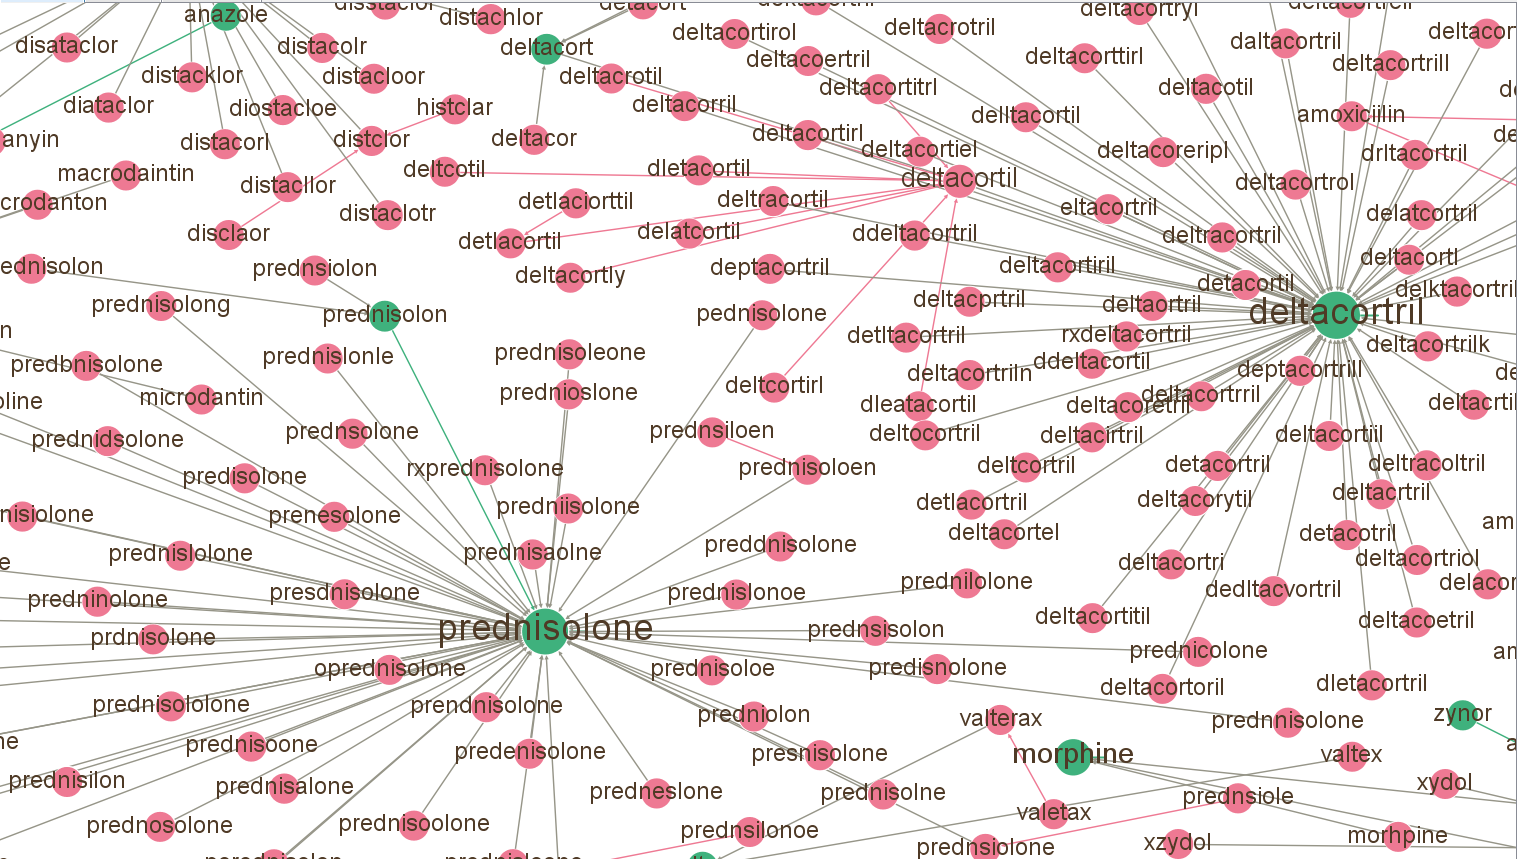
\includegraphics[width=\textwidth]{replace_drugs.PNG}
% where an .eps filename suffix will be assumed under latex, 
% and a .pdf suffix will be assumed for pdflatex; or what has been declared
\DeclareGraphicsExtensions.
\caption{Network simulation of correction decisions at a distance of two}
\label{network}
\end{figure*}

A network representation of this process can be observed in fig \ref{network}, where the edit distance is set to two. Green nodes represent correct candidate names, while red nodes represent incorrect ones. Node sizes represent the number of occurrences within the text.

As edit distances of three and four had had significantly inferior performance (relative to the number of errors generated) subsequent testing was conducted using edit distances of one and two. These edit distances were conducted on the previous results relating to edit distances of one or two, in order to explore whether increased accuracy could be generated by this process.



\begin{table}
\renewcommand{\arraystretch}{1.3}
% if using array.sty, it might be a good idea to tweak the value of
% \extrarowheight as needed to properly center the text within the cells
\caption{Second iteration of edit distance}
\label{table2}
\centering
\begin{tabular}{|c||c||c||c||c|}
\hline
initial step & second step & f$\rightarrow$t & t$\rightarrow$ t & t$\rightarrow$ f\\
\hline
\multirow{2}{*}{1} & 1 & 203 & 9  & 1   \\
\hhline{~----}
 & 2 & 568 & 95 & 11    \\
\hline
\multirow{2}{*}{2} & 1 & 84 & 11 & 3   \\
\hhline{~----}
 & 2 & 127 & 45 & 35  \\
\hline

\end{tabular}
\end{table}



The most successful route of edit distance correction involved an iterative process of correcting to a distance of two, and then correcting again to a distance of two on these results. 

This process left 728 correct pharmaceutical names out of a total of 977 candidate names. However, a substantial number of these medications appeared only once within the entire corpus. These 200 candidate single instance candidate names, which were predominantly incorrect (146 false to 34 true) could be discounted as outliers and removed. This left 685 true to 95 false candidate names: representing an overall accuracy of 88.15\%. When taking volume of occurrence into account, the retained candidate names represent an accuracy of 93.6\%

This final result represents an over 57\% rise in the precision of candidate names, from an initial accuracy of only 30.97\%. Of the initial 896 correct candidate names identified, 76.45\% were retained. However, if we discount outliers, this retention rises to 82.63\%. Looking at the numbers that the surviving candidates relate to, we see 359207 occurrences, of which 33599 relate to correct pharmaceutical names. However of this number  9870 instances relate to one correct pharmaceutical being wrongly corrected to another.

Taking a random sample of 200 records that were hand annotated by a domain expert for testing purposes, the program's training data achieved an 82.56\% recall. Of the pharmaceuticals correctly identified, 33.1\% were incorrectly spelled or written, of which 84.78\% were successfully corrected by the program, 15.21\% were unchanged and 2.17\% were incorrectly changed. Of the 76.9\% of the pharmaceuticals identified which had been correctly spelled, a further 2.15\%  were erroneously changed.

\section{Discussion}

The most apparent finding from the results is that automatic correction of pharmaceuticals necessitates very large volumes of data for accurate results. The greater the volume of data presented, the more likely that drugs will appear in the context of prescriptions and be caught by the information retrieval methods designed specifically to parse these structures. Moreover, the greater the volume of data collected, the easier it is to identify false positives and incorrectly recorded pharmaceuticals. 

While the contextual analysis performed relatively well in excluding unrelated domain-specific terminology from results, 11 of the final candidate pharmaceutical names were such terms (for instance `paediatric' and `suppos'). A possible solution to this would be to clean final results with a more extensive dictionary than that used in the course of this paper. It would not be advisable to use this larger dictionary to filter pharmaceuticals at the beginning of the collection process, as both abbreviations and variant spellings were clustered on these terms in the course of the program. However, the fact that 7 of these terms tend to appear in quite close proximity to prescription details may indicate a means of exclusion through contextual analysis. The 18 incorrect candidate names which represent misspelled English words (such as `injeciton', `depressent', and `strenght') may potentially be targeted in a similar manner.

%The program is fundamentally dependent on users predominantly writing correct versions of pharmaceuticals, and cannot account for particularly prevalent cognitive mistakes\cite{sessions2006effects}. For instance, a majority of users believed that amoxicillin was spelled amoxycillin in the corpus. This had the effect of inadvertently causing the correct version of the drug name to be clustered on the incorrect version. 

%Finally, in a handful of cases contracted forms of pharmaceuticals were longer than was originally expected, e.g. `fluclox' (for `flucloxacillin'). A relatively trivial solution is to automatically inflate candidate names which are affixes of longer alternatives. 

%While a conservative ceiling on edit distances will reduce the identification of false negatives,\cite{jupin2012understanding} there is no means to eliminate all possible false negatives without recourse to some sort of ontology.


\section{Conclusion}Using a predefined list of pharmaceuticals to develop a topographical understanding of context has proven a suitable means to discover pharmaceutical environments. However, while context has clear application in identification of medications within free-text notes, a more syntactically sensitive approach may yet yield stronger results in terms of both recall and precision. Nevertheless, the process exhibited in this paper has strong performance in both these categories. In particular, the capacity of the method described to discover hitherto unknown pharmaceuticals has obvious application. Non-trivial exclusion of false-positives is an ongoing concern. Furthermore, the method described does not itself provide any information about the relationships of true-positive pharmaceuticals to one another, and many different products may be recorded that have similar, or even identical functions.     

